\pagebreak
\begin{frame}{Grundlegende Theorie}{Definition}
    Im weitesten Sinne beschreibt ein Buffer Overflow eine Schwachstelle in einem Computerprogramm,
    bei der ein Angreifer einen Speicherbereich fester Größe überschreibt und diesen so zum “Überlaufen” bringt.
    Durch Ausspähen und Analysieren der Software kann dieses Überschreiben so gezielt geschehen, dass der Fluss des
    Programms verändert und zuvor injizierter Schadcode ausgeführt wird.    
\end{frame}


\begin{frame}{Grundlegende Theorie}{Speicheraufbau}
    \begin{figure}[h]
        \centering
        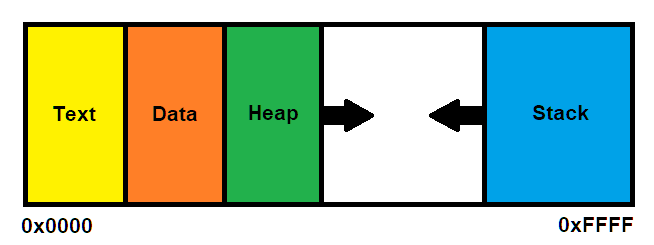
\includegraphics[width=0.7\textwidth,height=0.75\textheight,keepaspectratio]{images/process.png}
        \caption{Prozess im Speicher}
    \end{figure}
\end{frame}

\begin{frame}{Grundlegende Theorie}{Stack Overflow}
    \begin{itemize}
        \setlength{\itemindent}{19em}
        \item Wert einer Variable verändern
        \item Function Pointer manipulieren
        \item Return Pointer überschreiben        
    \end{itemize}
    \begin{figure}[h]
        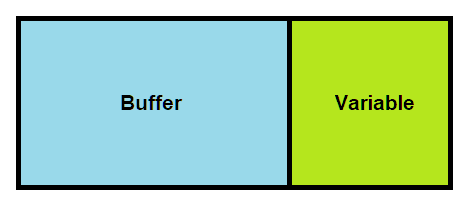
\includegraphics[width=0.475\textwidth]{images/buffer1.png}
        \hfill
        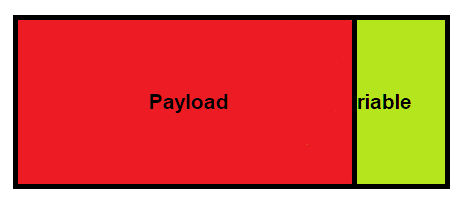
\includegraphics[width=0.475\textwidth]{images/buffer2.png}
        \caption{Buffer im Stack während eines Overflows}
    \end{figure}
\end{frame}



\begin{frame}{Grundlegende Theorie}{Weitere Overflows}
\begin{itemize}
        \item Heap Overflows
        \item Integer Overflows
        \item Unicode Overflows
    \end{itemize}
\end{frame}



